\section{Esempi d'utilizzo}
Di seguito vengono riportati alcuni esempi di utilizzo della nostra applicazione:

%
%
%
\subsection{Login/Registrazione}
L'accesso a questa sezione non richiede alcuna autenticazione preliminare. Gli utenti hanno la possibilità di effettuare la registrazione o il login per accedere alle funzionalità offerte.

\begin{figure}[htbp]
    \centering
    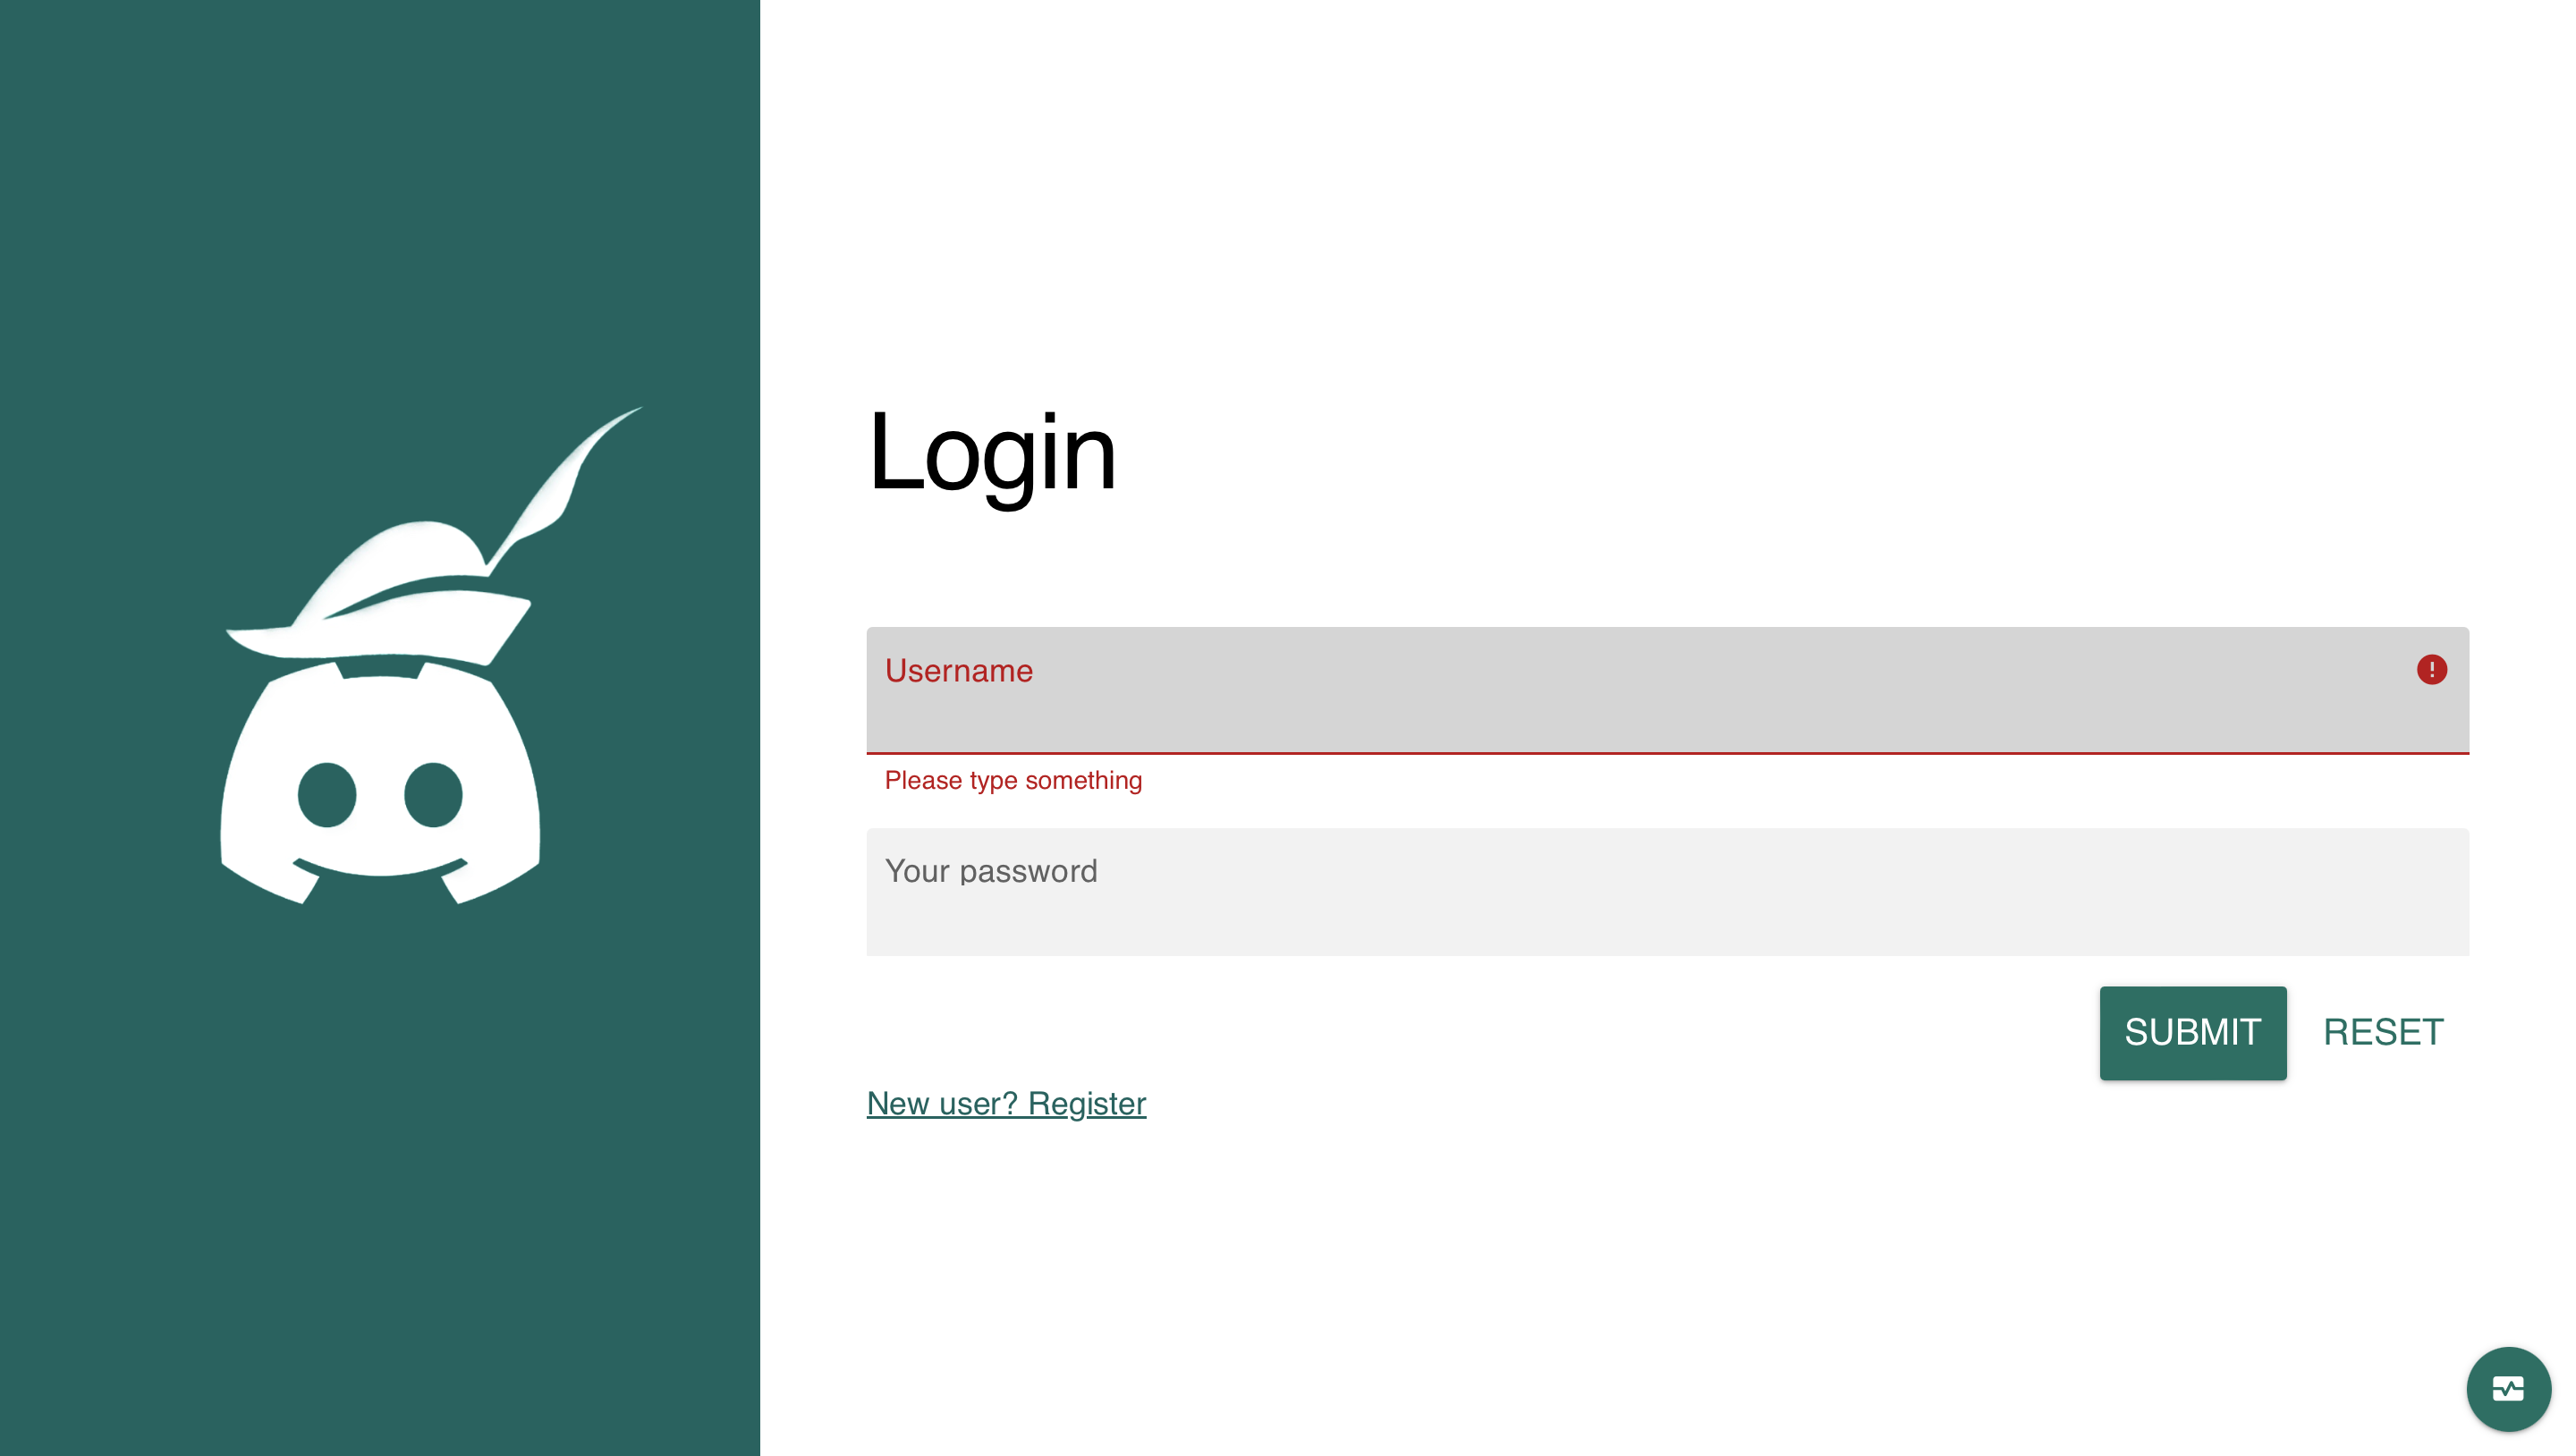
\includegraphics[width=0.9\textwidth]{sections/07-usage-example/img/Login.png}
    \label{fig:login_img}
\end{figure}


\begin{figure}[htbp]
    \centering
    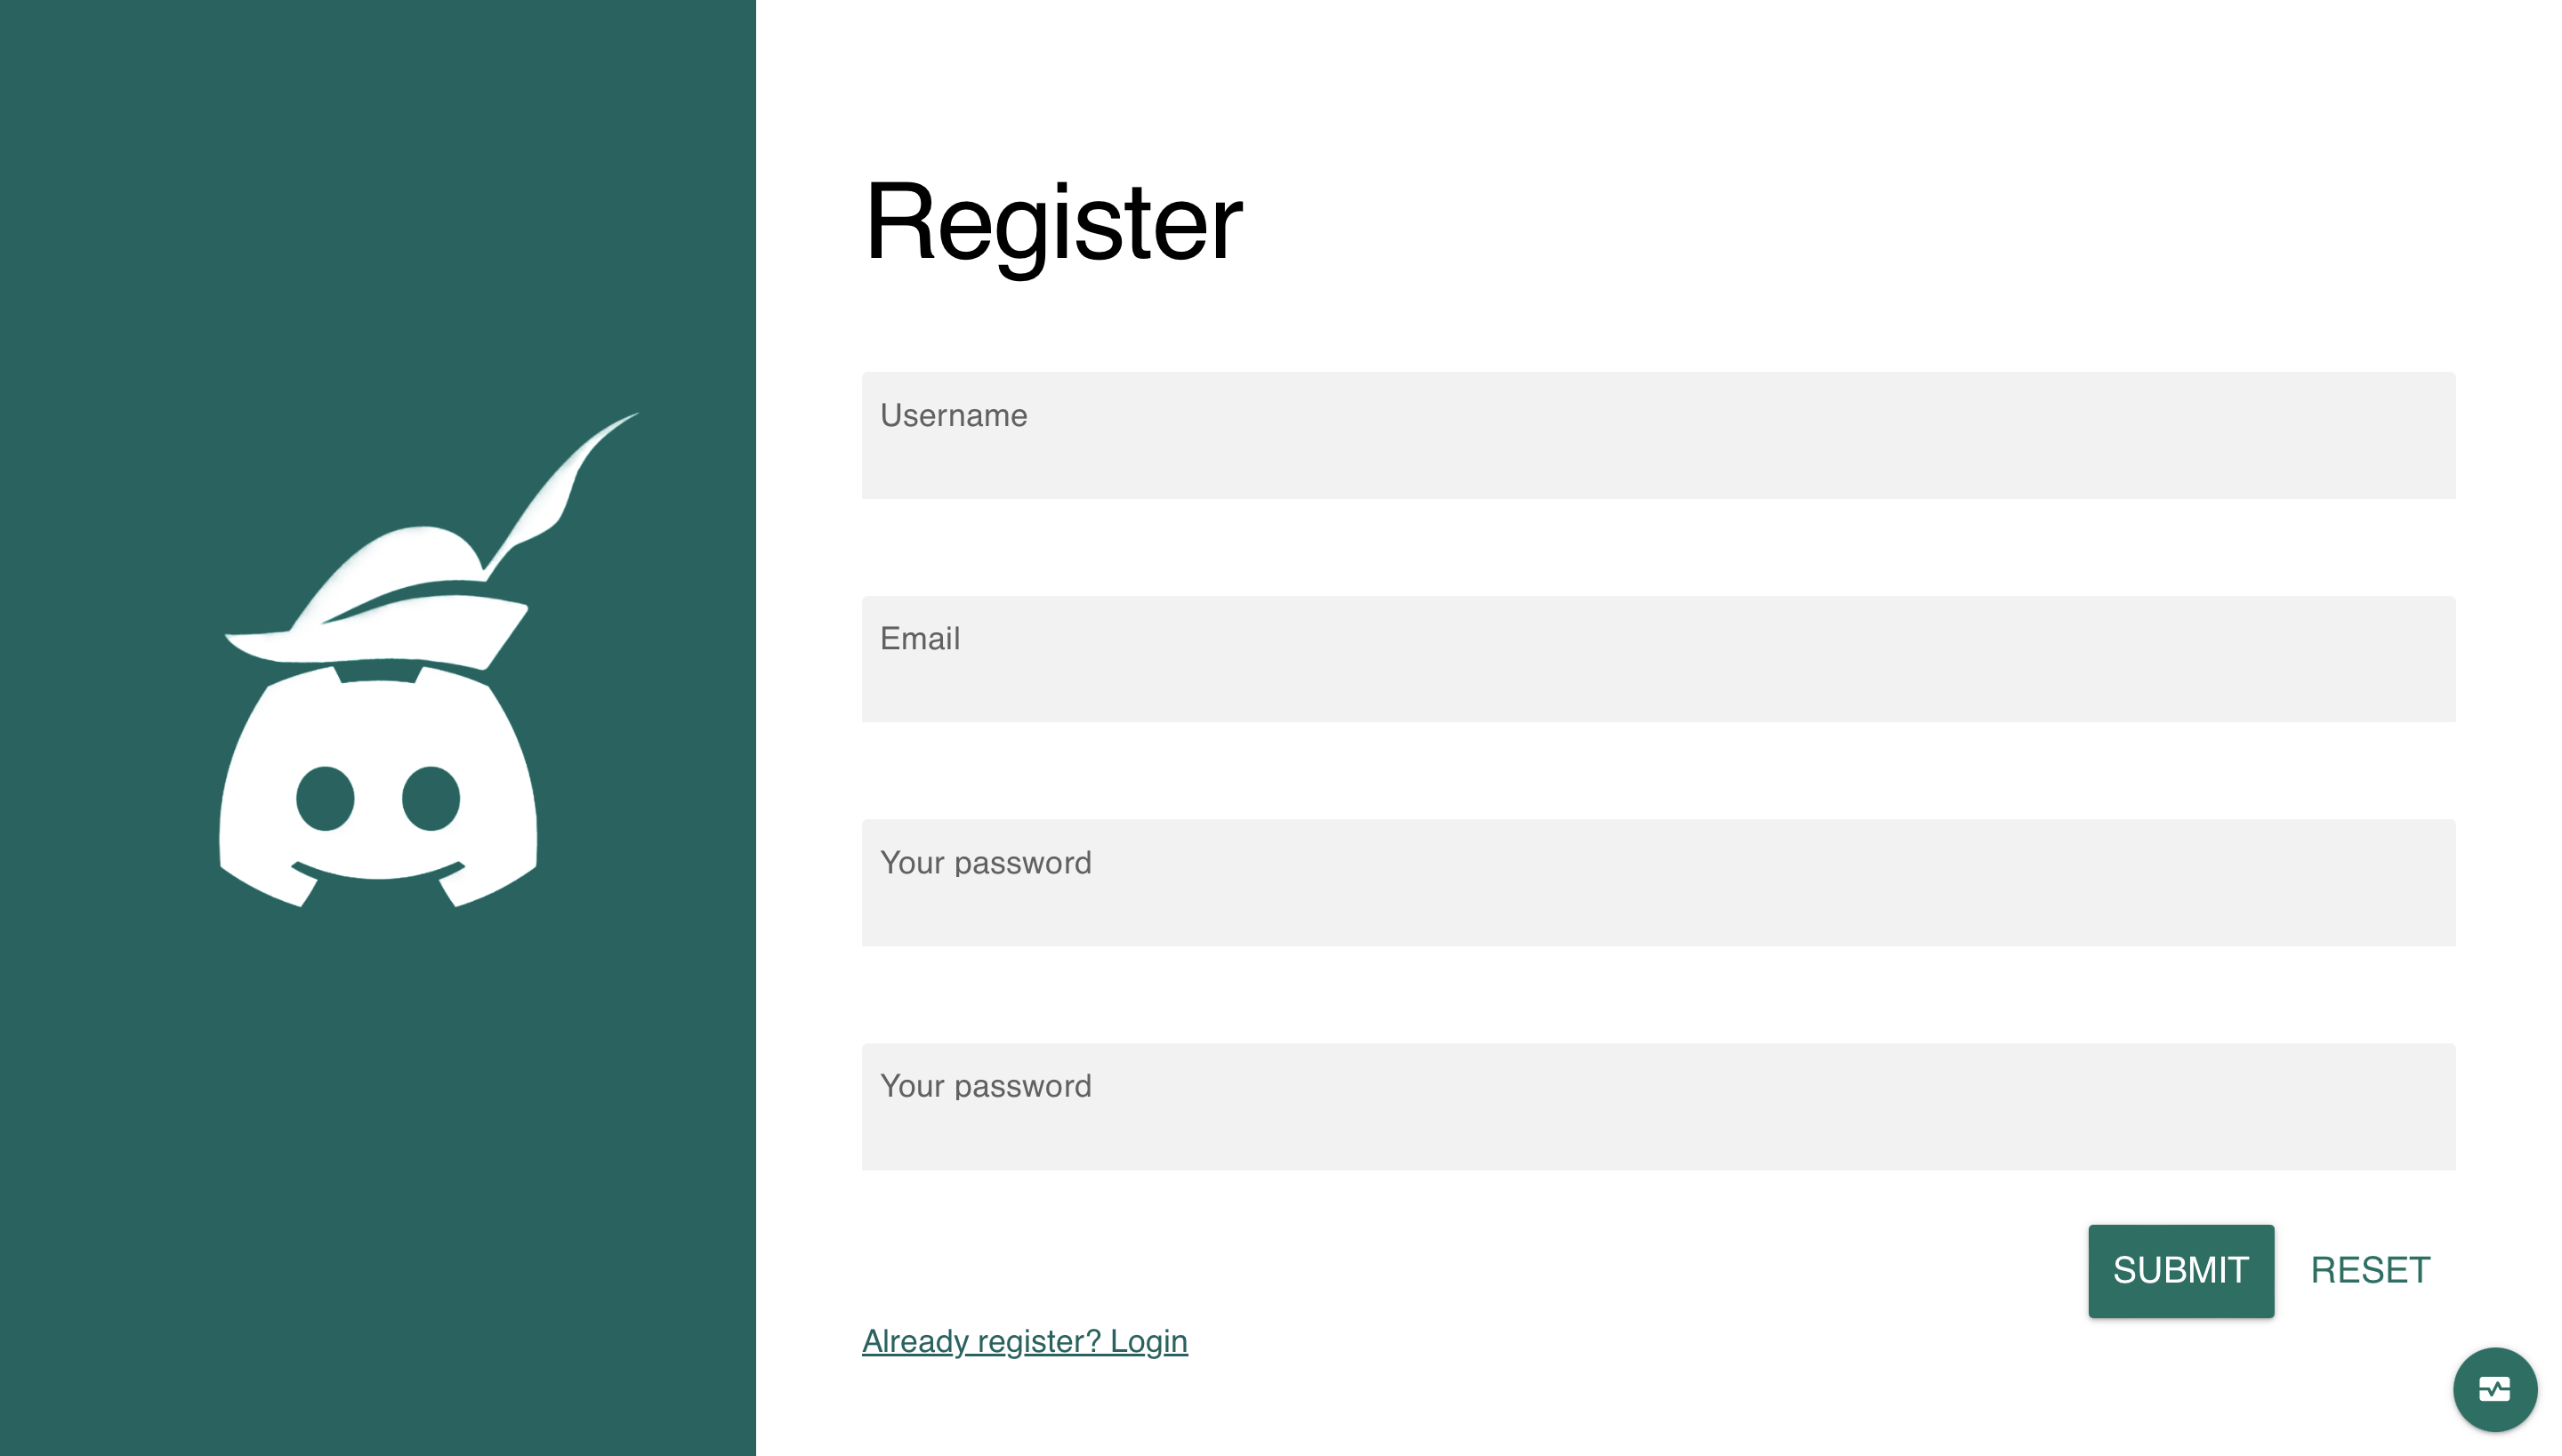
\includegraphics[width=0.9\textwidth]{sections/07-usage-example/img/Register.png}
    \label{fig:register_demo}
\end{figure}

%
%
%
\subsection{Monitoring/Healthcheck}
L'accesso a questa sezione è libero e non richiede credenziali di accesso. Qui gli utenti possono monitorare lo stato dei microservizi in modo rapido e semplice.

\begin{figure}[htbp]
    \centering
    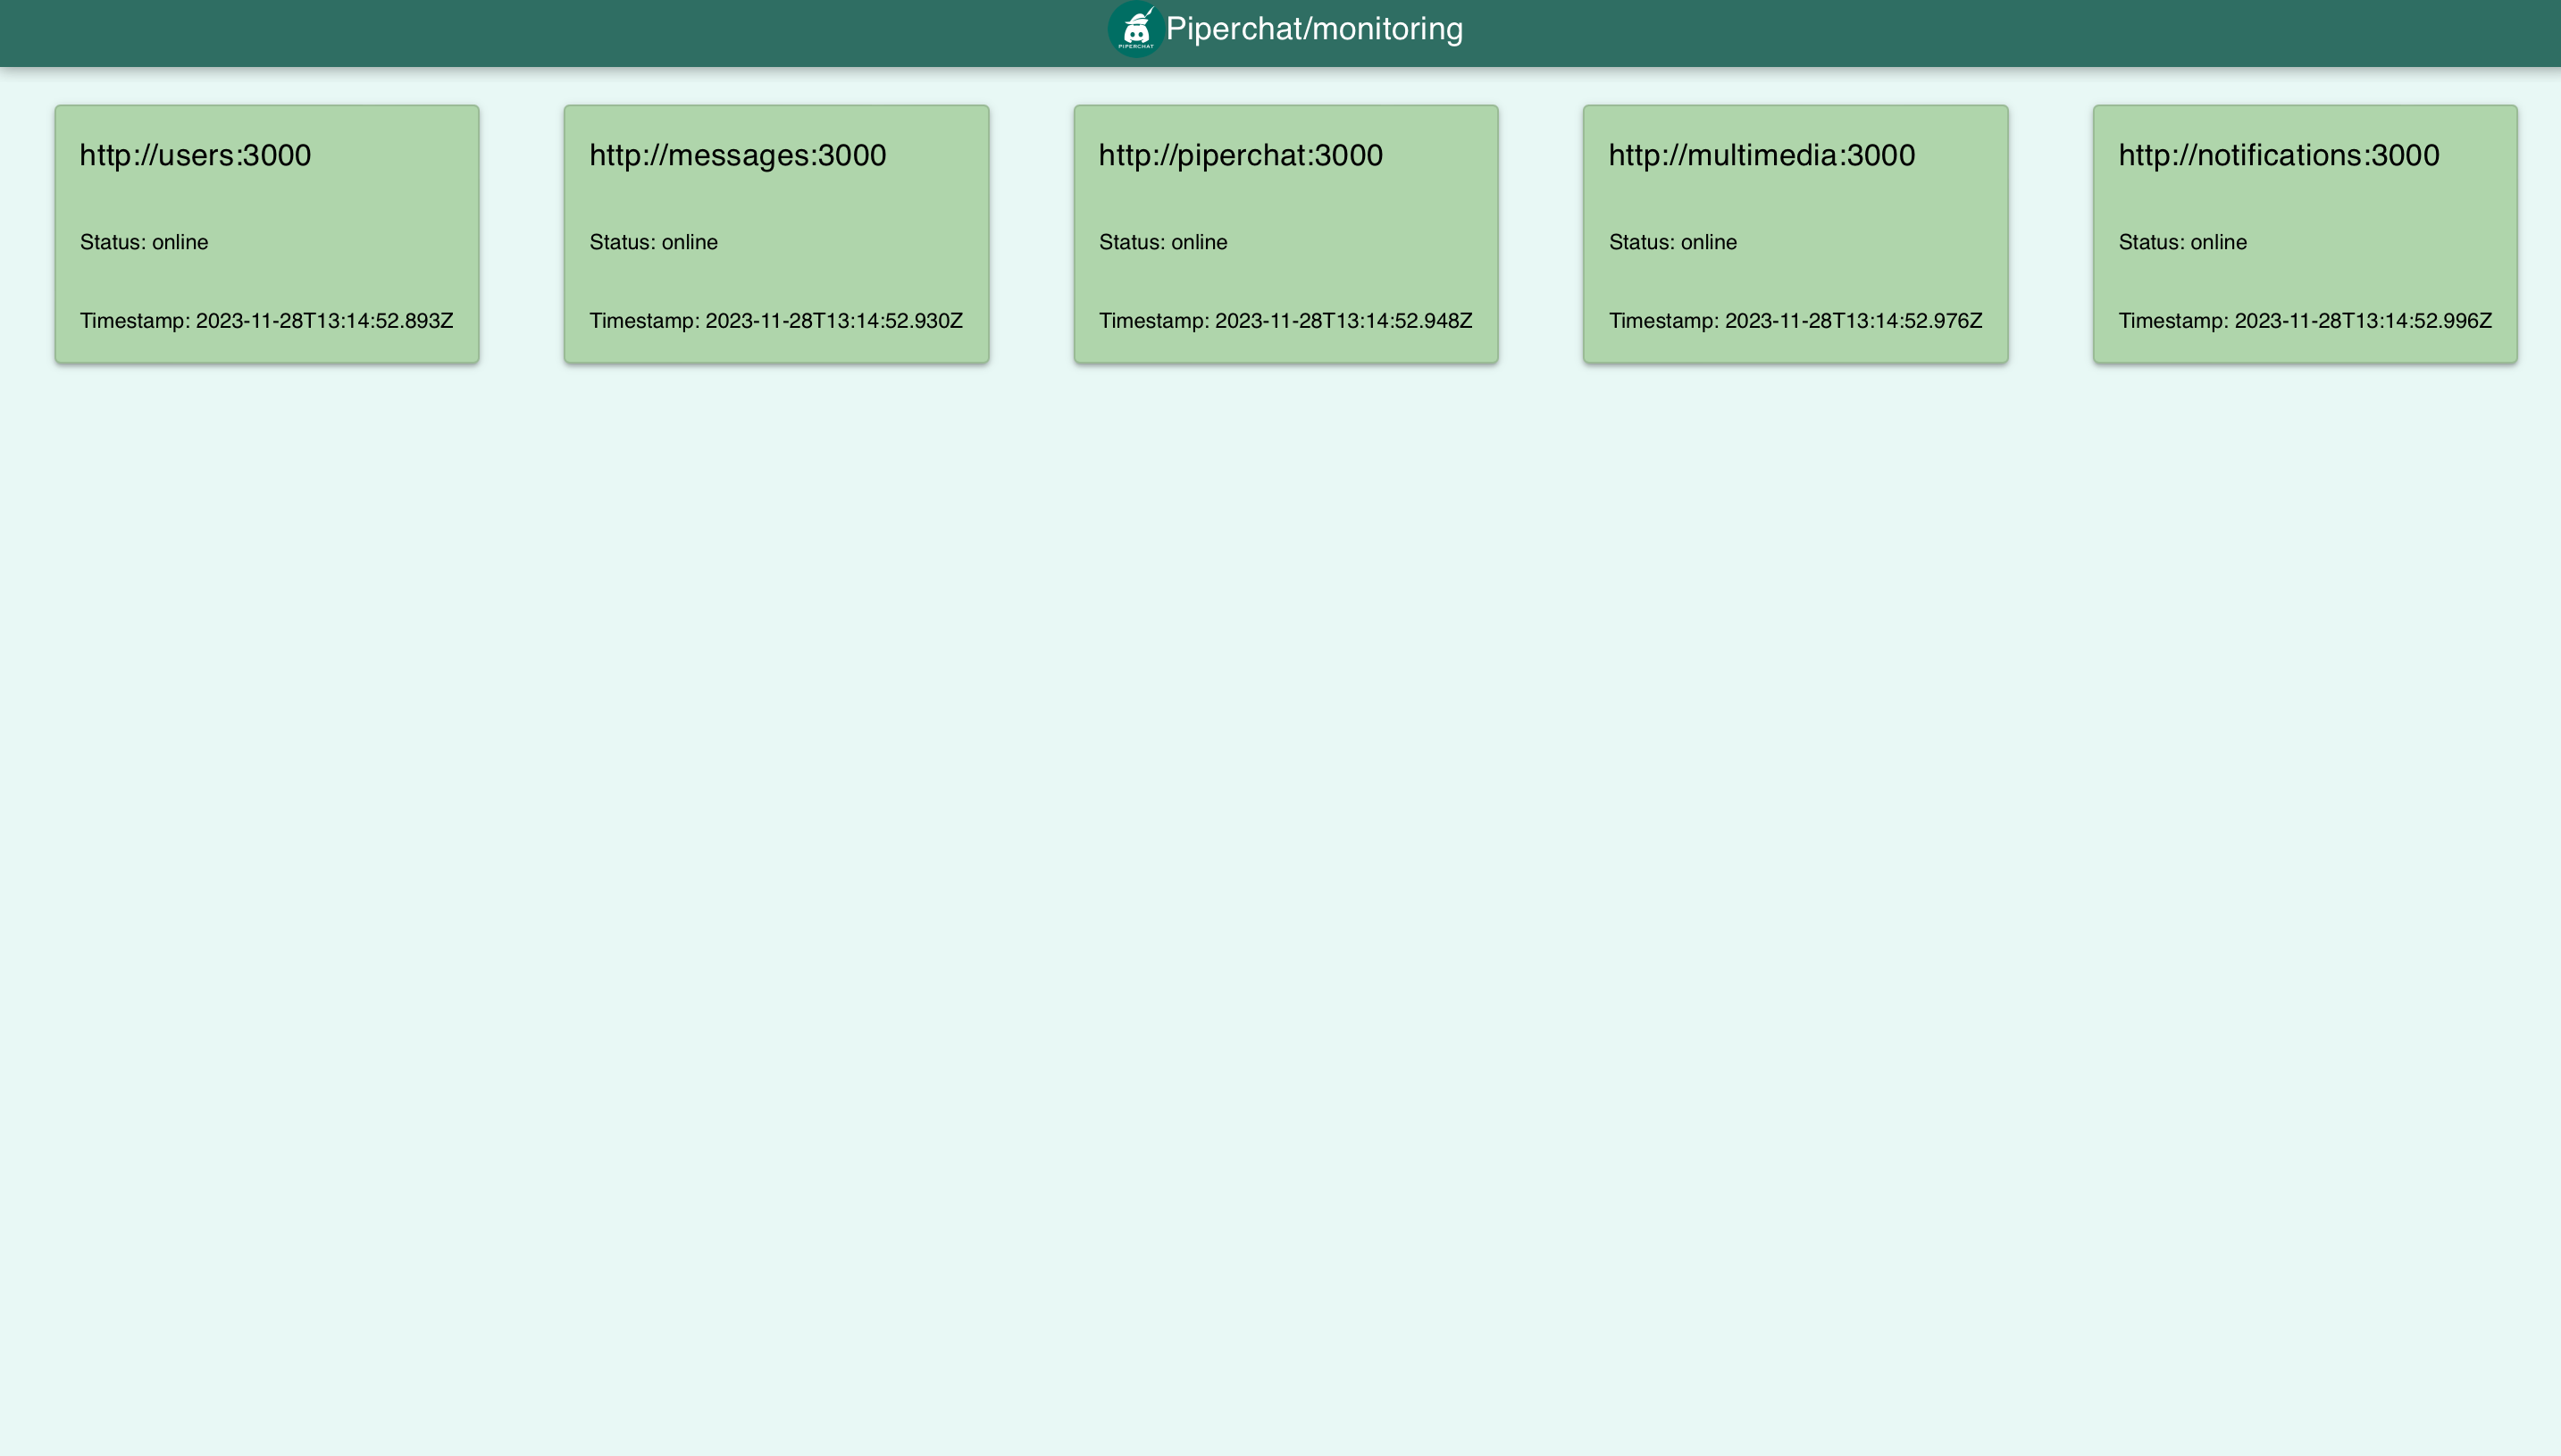
\includegraphics[width=\textwidth]{sections/07-usage-example/img/monitoring.png}
    \label{fig:moitoring_demo}
\end{figure}

%
%
%
\newpage
\subsection{HomePage}
Per accedere a questa sezione è necessario eseguire l'accesso. In caso di assenza di un access token valido, verrà automaticamente reindirizzati alla pagina di login. La struttura della pagina è articolata in due sezioni principali:
\begin{itemize}
    \item \textbf{Menù laterale}: Da qui è possibile navigare tra server, canali e messaggi diretti.
    \item \textbf{Area principale}: Questa sezione mostra i contenuti delle chat e delle videochiamate.
\end{itemize}

\begin{figure}[htbp]
    \centering
    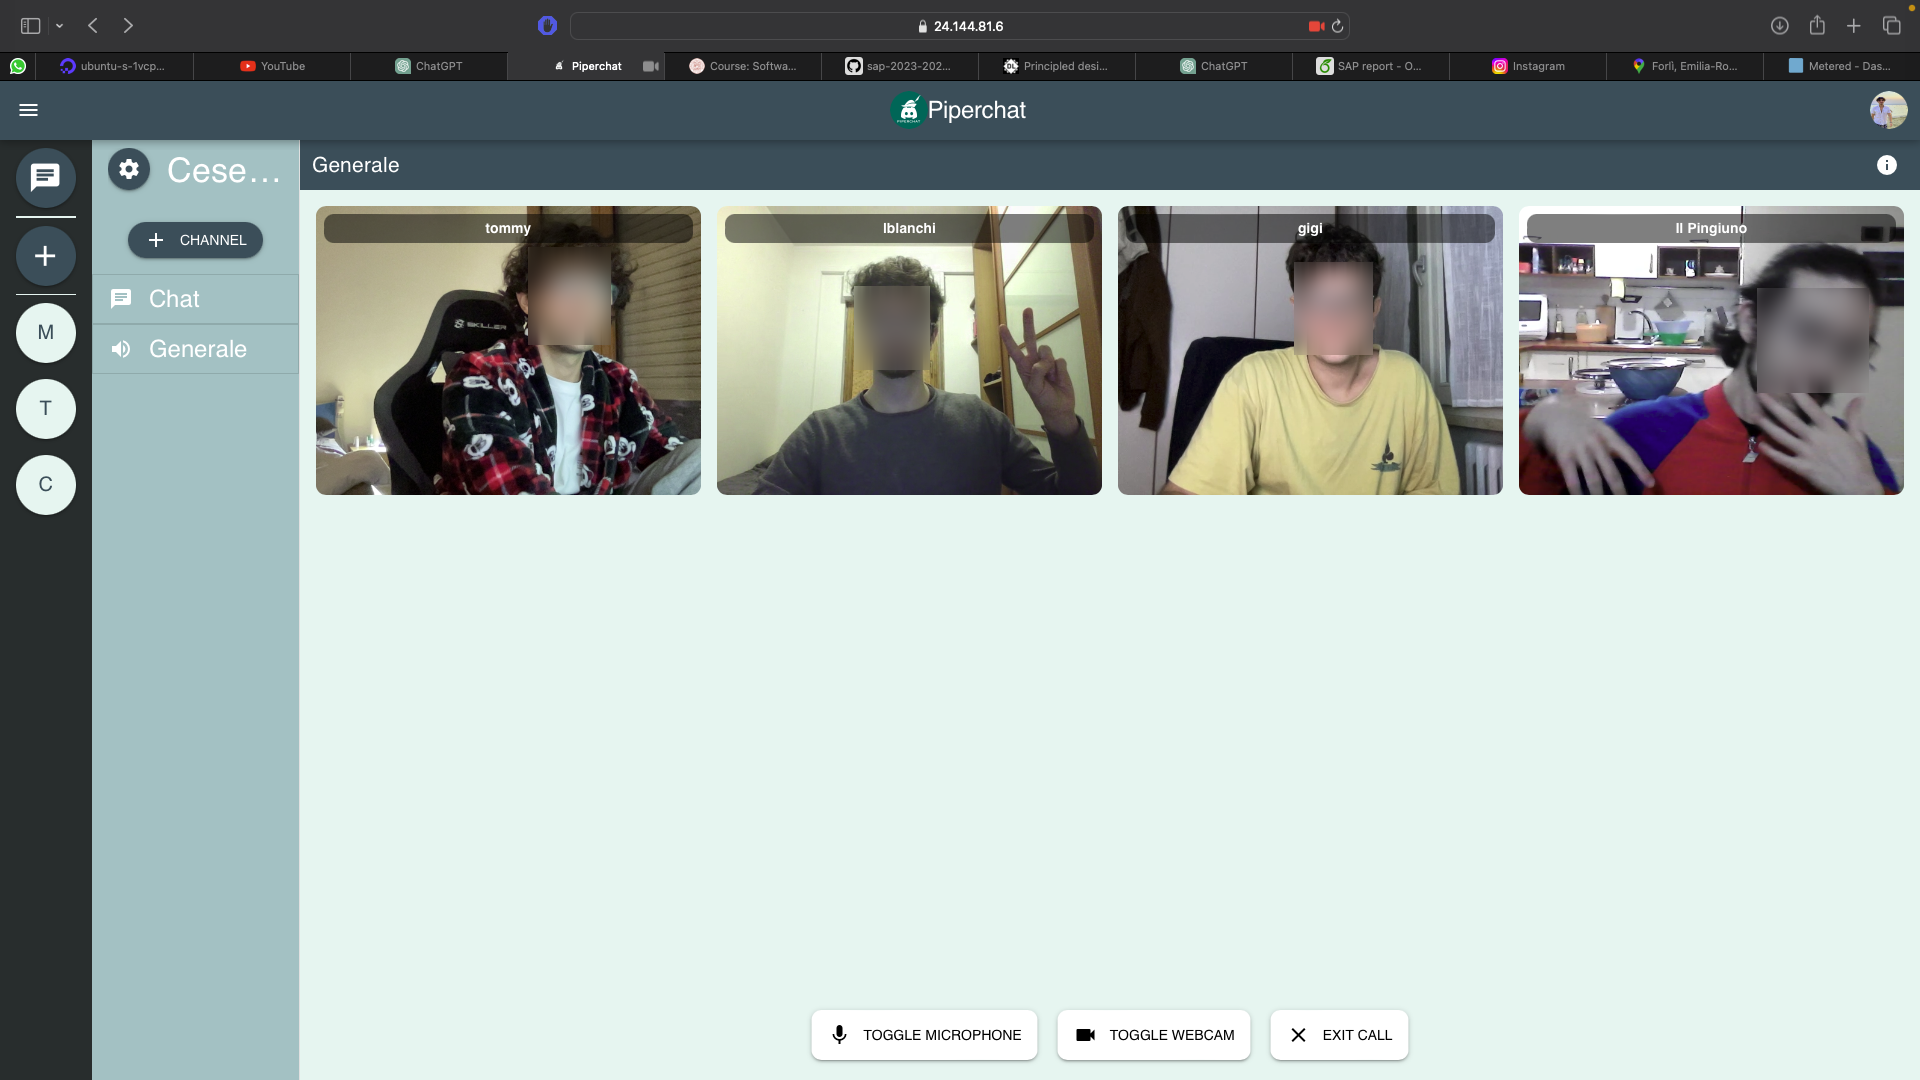
\includegraphics[width=\textwidth]{sections/07-usage-example/img/demo.png}
    \label{fig:webrtc_demo}
\end{figure}
